\documentclass[12pt,a4paper]{article}
\usepackage[english]{babel}
\usepackage[utf8]{inputenc}
\usepackage{amssymb,amsmath}
\usepackage[all]{xy}
\usepackage{url}
\usepackage{color}
\newcommand{\angstrom}{\textup{\AA}}
\color{black}
\usepackage[autostyle]{csquotes}
\usepackage{tikz}
\usetikzlibrary{bayesnet}
\def\UrlBreaks{\do\/\do-}
\usepackage{dcolumn}
\usepackage{booktabs}
\usepackage{tikz}
\usepackage{wrapfig}
\usetikzlibrary{positioning,shapes,arrows}
\newcolumntype{M}[1]{D{.}{.}{1.#1}}
\usepackage{upquote} % Upright quotes for verbatim code
\usepackage{fancyvrb} % verbatim replacement that allows latex
\usepackage{float}
\usepackage{wrapfig,lipsum,booktabs}
\usepackage{graphicx} 
\usepackage{animate}

\usepackage{amsmath}
\usepackage{algorithm}
\usepackage[noend]{algpseudocode}
\usepackage{listings}
\makeatletter
\def\BState{\State\hskip-\ALG@thistlm}
\makeatother
\usepackage{geometry}
\geometry{
	a4paper,
 	left=12mm,
 	right=12mm,
 	top=12mm,
 	bottom=15mm
}

\DefineVerbatimEnvironment{Highlighting}{Verbatim}{commandchars=\\\{\}}

\newcommand{\VerbatimStringTok}[1]{\textcolor[rgb]{0.25,0.44,0.63}{{#1}}}



\begin{document}
\title{Learning Sense Embeddings}
\author{Michał Ostyk-Narbutt (1854051)\\Prof. Roberto Navigli \\ Natural Language Processing Homework 2}

\maketitle


\begin{center}

\includegraphics[width=0.3\textwidth]{img/sapienza_logo.jpg}
\end{center}
\maketitle
\tableofcontents
\clearpage
\section{Introduction}
This report tries to present the process of learning sense embeddings from the annotated EuroSense corpus to be used on a word similarity task. 
%Section 2 presents the dataset and tools used for parsing, the model training approach along with a hyperparamter search. Section 3 depicts the results. Section 4 is a general discussion of the obtained results along with few interesting visualized cases. Finally section 5 concludes the work.
\section{Model and Approach}
\subsection{Dataset and tools}
The dataset used was the high precision version of the Eurosense corpus \cite{Eurosense}. It consists of a large \texttt{XML} file which consists of many multi-lingual sentences taken from the European Union parliament. All the processing steps used in this project were performed in Python 3, with he help of key external libraries. These were  \texttt{Gensim}  used for model training, \texttt{iterparse} used for parsing the large corpus, and \texttt{Scikit-Learn} for dimentionality. The code file structure can be found in the \texttt{README.md} file of the Gitlab repository \cite{code}.

\subsection{Parsing}
The parsing consisted of itertively reading the large corpus file, and processing it line by line. Using special tags, sentences were extracted along with their annotations. However, for the purposes of this assignment extraction was performed  only for the English language.
Each \textit{sentence}, consisted of several \textit{texts} for the English Language. However, not every \textit{text} had corresponding anchored annotations. Hence, these texts not containing any \textit{anchors} were discarded. Conversely, due to inconsistencies in the dataset, many sentences which had English \textit{anchor} annotations but lacked \textit{texts} were also discarded. Moreover annotations in this corpus file contain a certain ID called \textit{synsetID} which was specified in BabelNet. In this task, only annotations which had a corresponding \textit{synsetID} in WordNet were considered.
\begin{wrapfigure}[16]{r}{0.5\textwidth}
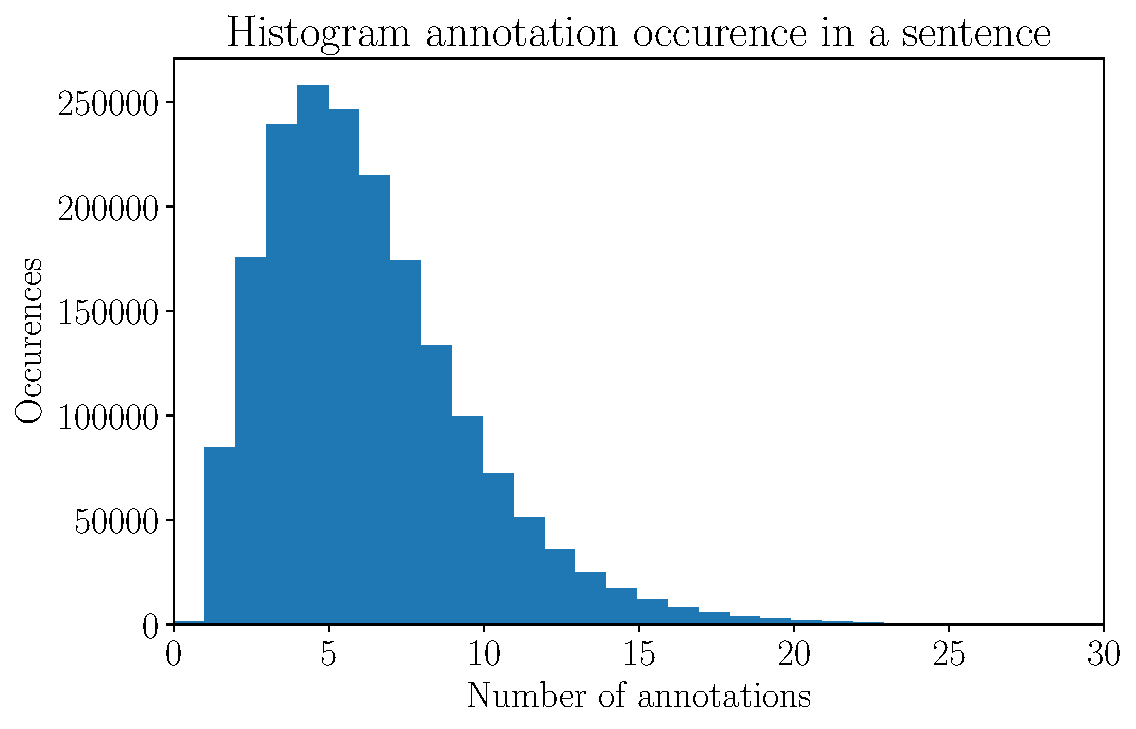
\includegraphics[width=0.5\textwidth, angle = 0]{img/annotations.pdf}
\caption{Histogram based on the number of annoations in each of the 1.87 m extracted sentences}
\vspace{-25pt}
\label{img:parsed}
\end{wrapfigure}
Stop words were \textbf{not} removed, but certain punctuation marks were as they conflicted with some anchors. For example: "European Union-Ukraine Agreement", were there was an anchor for "European Union". Additionally prior to writing the parsed sentences to file, they were lowered as not to have duplicates of senses  ie.:  "\textbf{l}emma$\_$synsetID" and "\textbf{L}emma$\_$synsetID".
In total, $1.87$ million sentences were extracted from the dataset. 
Figure \ref{img:parsed} portrays a histogram of annotation occurrences in each parsed sentence. The median number of annotation was \textbf{5}. This could be an indicator of how word senses affect each other depending on the number of annotations. In total, $1.87$ million sentences were extracted from the dataset.

\subsection{Training}
The training was performed using the the Word2Vec model from \texttt{gensim}.  At first, only the $CBOW$ version was used, but at the end $SKIPGRAM$ was implemented for comparison.

\subsubsection{Scoring: Similarity measure}
A key target of training the model, was to evaluate it on a similarity measurement task. For this, I utilised cosine similarity between words. Then using Spearman correlation, I tested the results against a gold, human-annotated dataset. I did not incorporate any other similarity measures. 

\subsubsection{Hyperparmeters}
The key hyperparamters explored when training the model were: $\alpha$ $-$ learning rate, min count $-$ minimum count of word occurrence in the vocabulary (of the parsed dataset), window, and the embedding size. These hyperparameters were explored using grid search in order to maximize the correlation score.
\begin{wraptable}[8]{r}{0.5\textwidth}
\vspace{-25pt}
\caption{Table of hyperparemters used in the grid search with best ones in bold}\label{wrap-tab:1}
\centering
\begin{tabular}{|c|c|c|}
\hline
window & 4 & \textbf{5} \\ \hline
min count & 1 & \textbf{3} \\ \hline
embedding size & \textbf{100} & 300 \\ \hline
$\alpha$ & 0.001 & \textbf{0.009} \\ \hline
Negative & \multicolumn{2}{c|}{\textbf{13}} \\ \hline
Epochs & \multicolumn{2}{c|}{\textbf{50}} \\ \hline
\end{tabular}
\end{wraptable} 
As for for the grid search, I implemented a \texttt{Word2VecModel} class, which resembles a \texttt{scikit-learn} estimator. It consists of a \texttt{fit} function which builds the model, given a set of hyperparameters, then builds the vocabulary, and proceeds to train it on a set number of epochs (50). Then using \texttt{sklearn.model.selection.ParameterGrid}, I iteratively perform a grid seach of the best hyperparameters based on the cosine similarity score performance.



\section{Results}

Since $CBOW$ works several times faster to train than skipgram, it was used for the grid search.
Grid search was first performed on large number of combinations of hyperparamters, on 15 epochs. However, after noticing significant discrepancies in the correlation score, a selected few were selected to be trained in the final grid search. The hyperparamters are presented in Table \ref{wrap-tab:1}, and the ones in bold refer to the best result of correlation $= 0.27$ (using $CBOW$). Using these best hyperapameters, a $SKIPGRAM$ version of the word2vec model was also trained and resulted in a slightly worse of correlation $= 0.26$. The difference in performance seems consistent with the fact that $CBOW$ has slightly better accuracy for the frequent words, since we used a min count of 3 but $SKIPGRAM$ works better with rare phrases. A more graphical approach to visualizing the effect of hyperparamters on each other, and the ones which have the most effect on the final score is presented in Figure \ref{img:grid}. The figure presents a swarm plot of the correlation score in regards to the hyperparamters. 

\begin{figure}[h]
\begin{center}
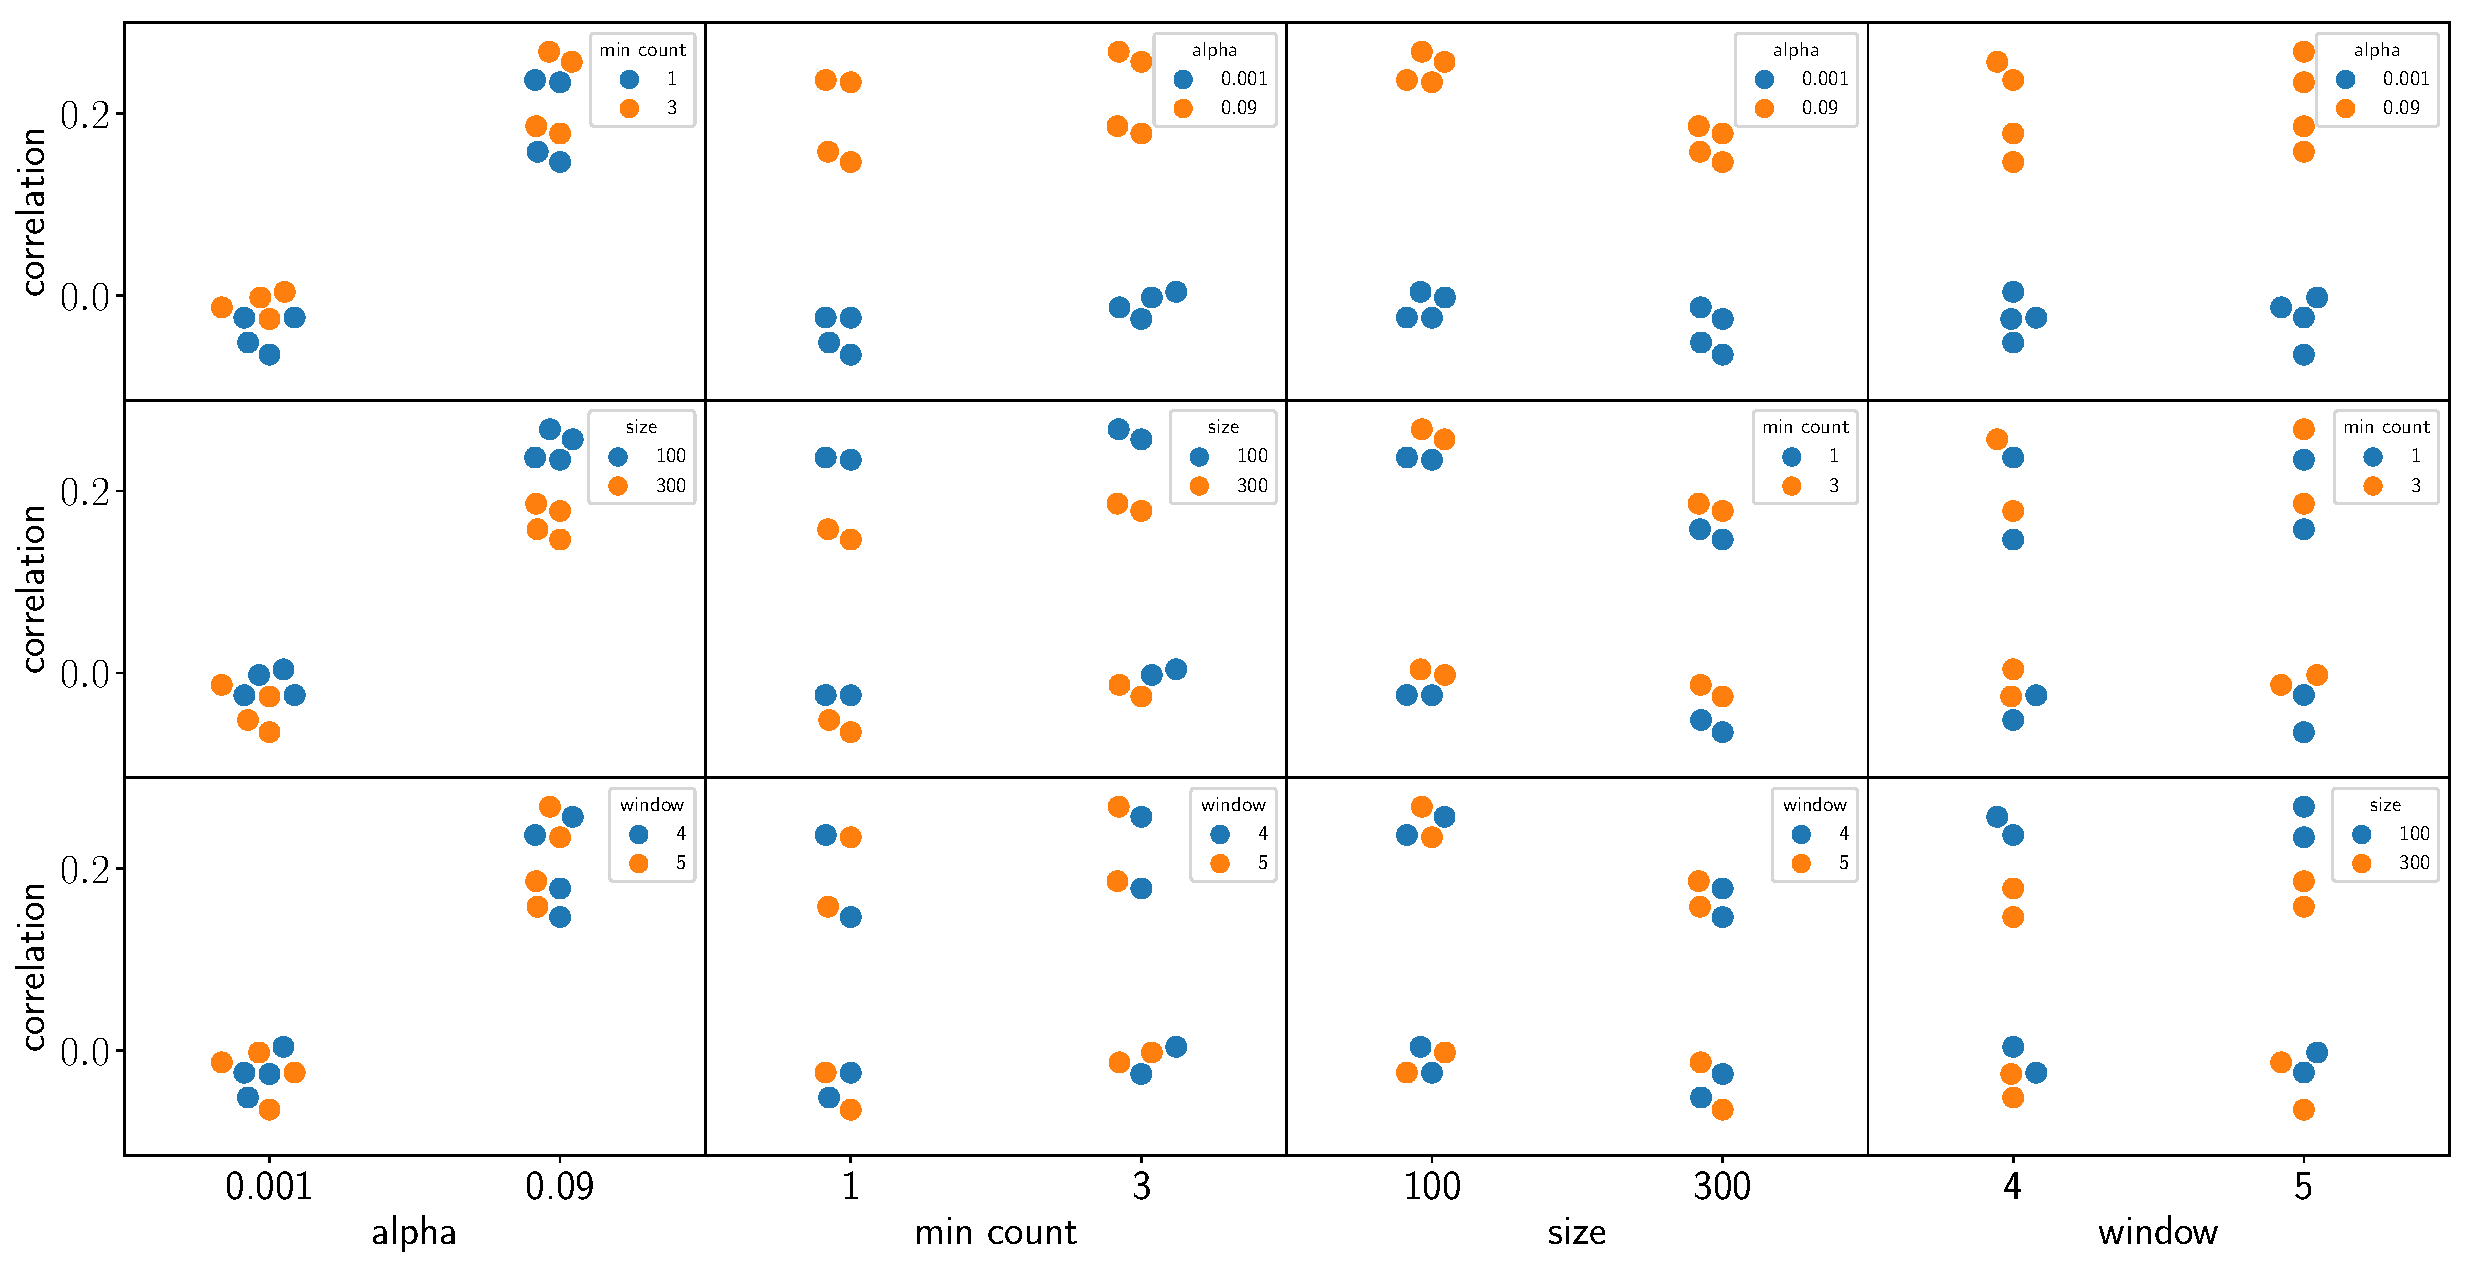
\includegraphics[width=\columnwidth, angle = 0]{img/grid.pdf}
\end{center}
\caption{Grid search of the best hyperparamters based on Table \ref{wrap-tab:1}. Visualization of the Correlation score vs each parameter depending on several others.}
\label{img:grid}
\end{figure}
 
\section{Discussion}

\subsection{General}
From Figure \ref{img:grid}, we can infer that alpha $\alpha$, has the most significant impact on the final correlation score, as regardless of the comparing hyperparamter, $\alpha = 0.09$ always yields a better correlation score.  Moreover, the difference is so substantial that for $\alpha = 0.001$ correlation scores swarm around 0, which would infer almost the lack of correlation. Additionally, we can see that the size of the embedding also plays a major role, as smaller (100) embeddings perform much better than larger (300). This is a consequence of the size of the vocabulary which is effected both by the min count parameter, but also more importantly by the contents of the corpus. 

The corpus is very domain specific which influences correlation scores, with its context and also results in many out-of-vocabulary (OOV) words. A possible solution would be to simply add data from a wider domain, including non factual texts like novels. 
This however is not easy, as finding enough annotated data is quite difficult but could be partially overcome by combining the already made synsets and analysing them in different ways. On the other hand, it would be far safer to use  a good corpus for a more wider domain, i.e:  the Semantically Enriched Wikipedia (SEW) \cite{sew} corpus.

Furthermore, the overall performance of the model could be yet improved by considering the rising problem of sparsity in the data. One key driving factor of sparsity is the reduction of polysemy which yields a large number of synsets. To overcome this, one could possibly reduce the number of senses for a given lemma but different synset.

\subsection{Embedding visualization}
To further understand what kind of embeddings \texttt{word2vec} produces, embedding visualizations were performed. To do this, I reduced their dimensionality from $size = 100$ to 2D and 3D using the \texttt{sklearn} implementation of Principal Component Analysis (PCA) followed by T-distributed Stochastic Neighbor Embedding (t-SNE) and removed synset IDs  for plotting purposes.

Figure \ref{img:tsne2D} depicts a 2D plot of a few chosen word embeddings (legend) and their top 30 most similar words according to the model.  From the depicted 4 words we can deduce that they are some are more closely matched than others. Whereas Figure \ref{img:tsne3D} portrays a 3D visualization of all the 44 thousand words in the vocabulary of the model. The plot is basically just one giant cluster in 3D symbolizing that on a larger scale, how much of a domain-specific dataset Eurosense really is.

\begin{figure}[h]
\begin{center}
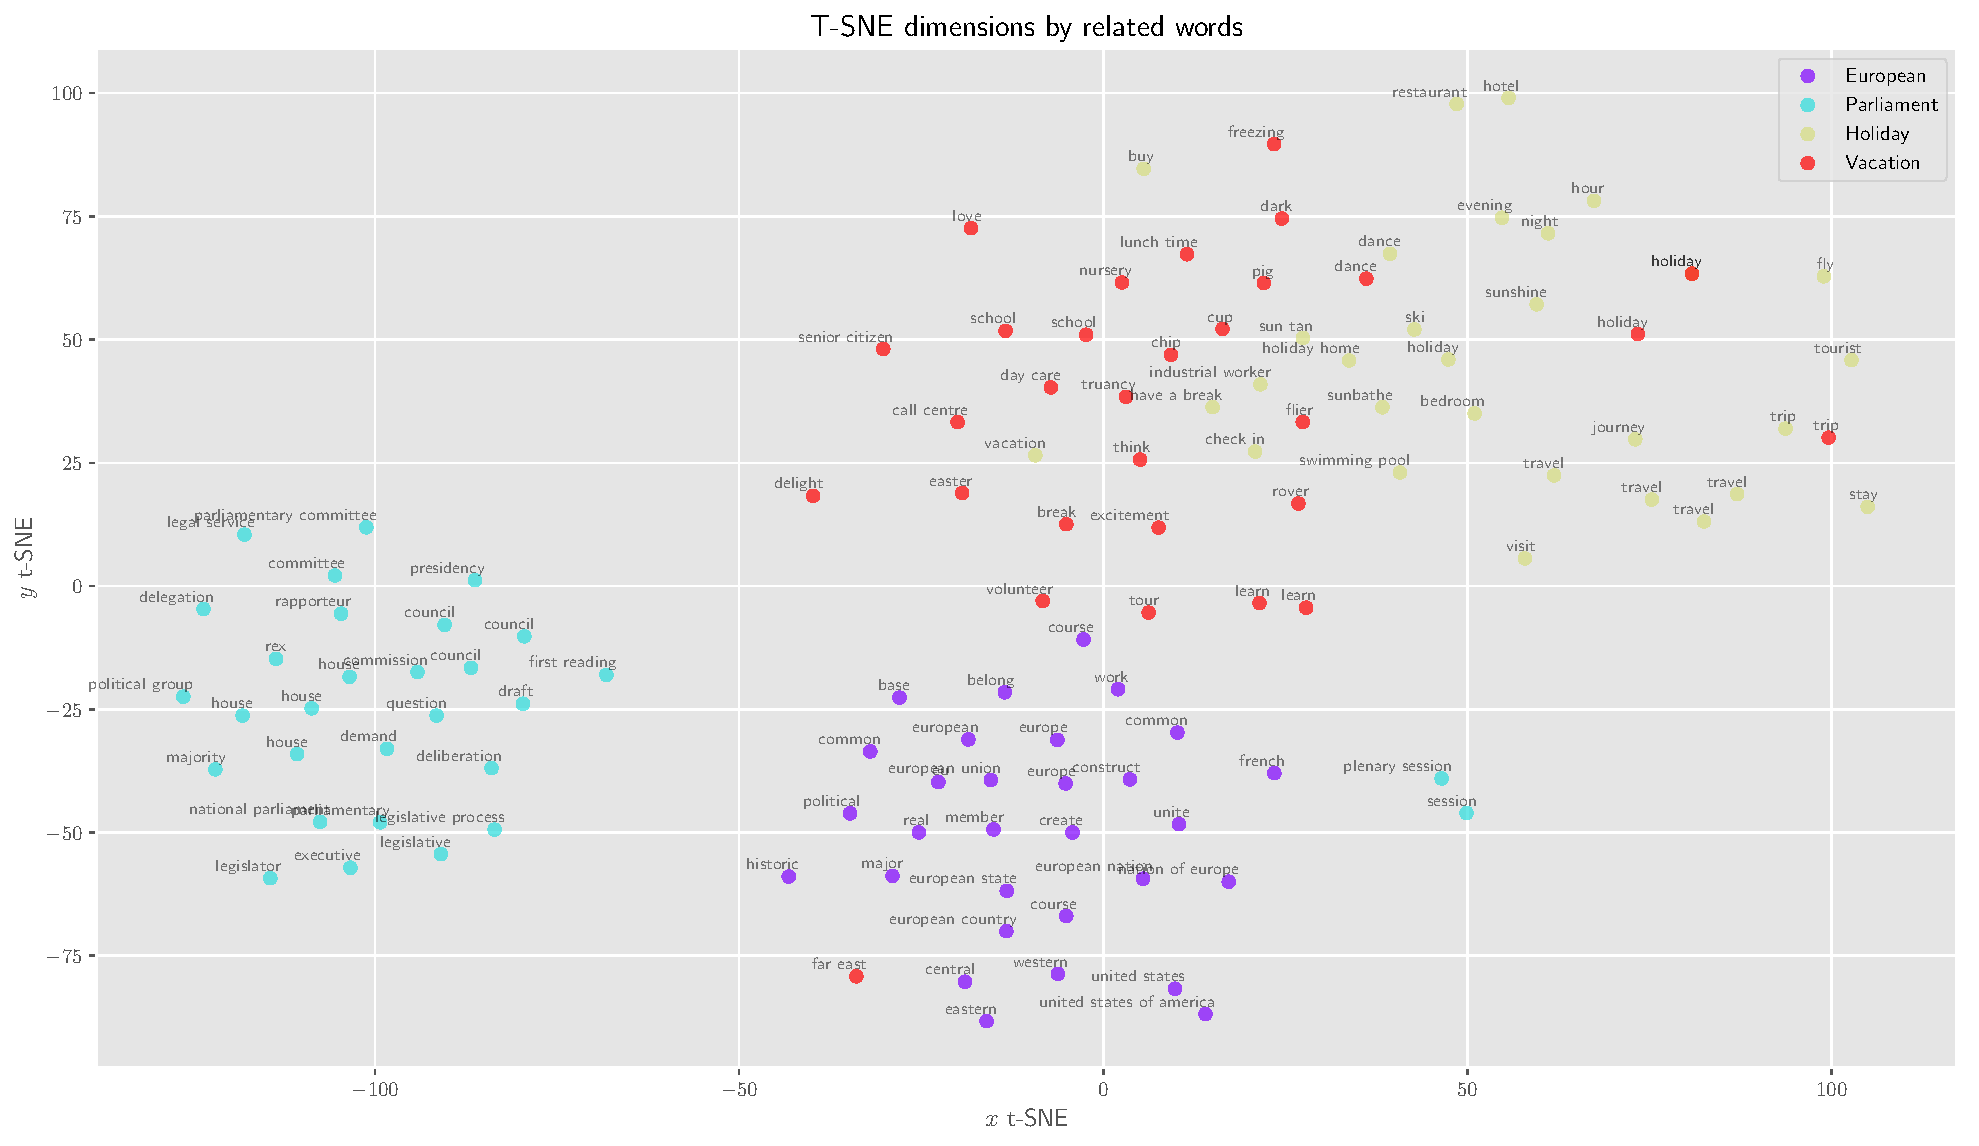
\includegraphics[width=\columnwidth, angle = 0]{img/tsne2D.pdf}
\end{center}
\caption{T-SNE visualization of the top 30 similar words to 'European' , 'Parliament', 'Holiday', and 'Vacation' . T-SNE with $perplexity = 20$ and $n\_iter = 5000$. Plots inspired by \cite{tsne}}
\label{img:tsne2D}
\end{figure}

\begin{figure}[H]
\begin{center}
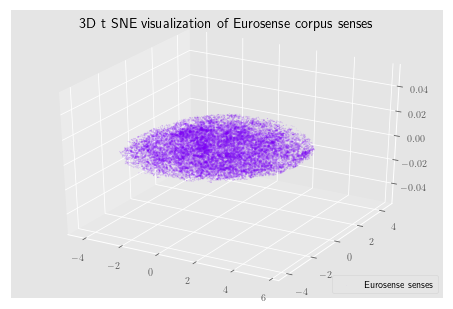
\includegraphics[width=0.5\columnwidth, angle = 0]{img/tsne3D.png}
\end{center}
\caption{3D T-SNE on the entire vocabulary of the model. $Perplexity = 3$ and $n\_iter = 300$. First reduced by PCA to 10 dimensions then applied T-SNE on 10 nearesst neighbours. Plots inspired by \cite{tsne}}
\label{img:tsne3D}
\end{figure}
%\includemovie{1cm}{1cm}{img/tsne.gif}
%\includegraphics[height=2.8in,autoplay,controls]{12}{img/imgpdf/animate_}{0}{120}
%TSNE PLOTS
%\begin{center}
%\animategraphics[height=2.8in]{12}{imgpdf/animate_}{1}{28}
%\end{center}
\section{Conclusion}
The best model, when stacked on a word similarity task yielded a correlation score of $= 0.27$. This score, could possibly be futher improved by a couple of factors. Namely, adding more data from more general and less domain dependent datasets. However, this arising issue of sparsity would also have to addressed in that case. Moreover, in the task similarity task, the OOV words significantly decreased the correlation score as there were OOV words in 48 out of the 353 pairs of words analyzed. To conclude, sense embeddings are an effective way of dealing with polysemy.  In this approach we created sense embeddings though anchoring specific synsets to lemma's of words in text. 
The world similarity measurement which compares our results with manual human scoring should yield far better results, as almost always the case in Deep Learning,  with more and better data.

\begin{thebibliography}{1}

\bibitem{Eurosense} Claudio Delli Bovi, José Camacho Collados, Alessandro Raganato and Roberto Navigli.
EuroSense: Automatic Harvesting of Multilingual Sense Annotations from Parallel Text. Proceedings of 55th annual meeting of the Association for Computational Linguistics (ACL 2017), pages 594–600, Vancouver, Canada, 30 July-4 August 2017. \url{http://lcl.uniroma1.it/eurosense/}

\bibitem{sew} Alessandro Raganato, Claudio Delli Bovi and Roberto Navigli.
Automatic Construction and Evaluation of a Large Semantically Enriched Wikipedia. Proceedings of 25th International Joint Conference on Artificial Intelligence (IJCAI-16), pages 2894–2900, New York City, New York, USA, 9-15 July 2016. \url{http://lcl.uniroma1.it/sew/}

\bibitem{tsne} \url{https://github.com/sismetanin/word2vec-tsne}
\bibitem{code} \url{https://gitlab.com/Ostyk/michal_ostyknarbutt_1854051_nlp19hw2}
\end{thebibliography}

\end{document}
